\documentclass[12pt]{article}
\usepackage[margin=0.75in]{geometry}
\usepackage{graphicx}
\setlength{\parindent}{0mm}

\begin{document}

{\centering
\large Math Practice \par
}
\hfill \break

Problems 1-3 - Solve the equation for $x$ using the following techniques:
(a) symbolically with paper and pencil,
(b) using the SageMath software, and
(c) graphically by setting the left-hand-side equal to $y_1$ and the right-hand-side equal to $y_2$ and seeing where the two lines intersect. \\ \\
1) $10 - 5(x+3) = 3x - 9$ \\ \\
\underline{Solution} $-$ \\
(a) Distribute the $-5$ to the $x$ and the $3$:
\begin{center}
$10 - 5x - 15 = 3x - 9$
\end{center}
Bring like terms to the same side of the equation and combine them:
\begin{center}
$4 = 8x$
\end{center}
Divide both sides by $8$:
\begin{center}
$x = \frac{1}{2}.$
\end{center}
(b) Run the following SageMath script:
\begin{verbatim}
x, y1, y2 = var("x y1 y2")
y1 = 10 - 5*(x + 3)
y2 = 3*x - 9
solve([y1 == y2], x)
\end{verbatim}
(c) Run the following SageMath script:
\begin{verbatim}
p1 = plot(y1, (x, 0, 2), color="red")
p2 = plot(y2, (x, 0, 2), color="blue")
g = Graphics()
g += p1
g += p2
g.show()
\end{verbatim}

\pagebreak

2) $\frac{6}{x+2} + \frac{2}{x-4} = \frac{-7}{x^2 - 2x - 8}$

\pagebreak

3) $x^2 + 5x = -1$

\pagebreak

4) Find an equation for the line that passes through the points $(-2, 3)$ and $(6, 7)$.

\pagebreak

Problems 5-6 - Solve the system of equations using the following techniques:
(a) symbolically with paper and pencil, and
(b) using the SageMath software. \\ \\
5) $3.5x + 4.1y = -18$, $6.2x - 11.5y = 30$ \\ \\
\underline{Solution} $-$ \\
(a) Solve the first equation for $y$:
\begin{center}
$y = \frac{-16 - 2.5x}{3.1}$
\end{center}
Plug this into the second equation:
\begin{center}
$5.2x - 10.5 \left( \frac{-16 - 2.5x}{3.1} \right) = 29$
\end{center}
Solve this for $x$:
\begin{center}
$x = -1.28$
\end{center}
Now use this $x$ to solve for $y$:
\begin{center}
$y = \frac{-16 - 2.5(-1.28)}{3.1} = -3.30.$
\end{center}
(b) Run the following in SageMath:
\begin{verbatim}
x, y = var("x, y")
solve([3.5*x + 4.1*y == -18, 6.2*x - 11.5*y == 30], x, y)
\end{verbatim}

\pagebreak

6) $55.3x - 12.5 = 9.7y + 3.1$, $5.2y = 8.8x - 22.6$

\pagebreak

7) Find the unknown sides and angle of the right triangle shown below.
\begin{figure}[!h]
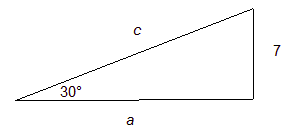
\includegraphics[scale=0.8]{figures/rightTriangle.png}
\end{figure}

\pagebreak
8) A pole leans away from the sun at an angle of $7^\circ$ to the vertical, as shown below.
When the elevation of the sun is $55^\circ$, the pole casts a shadow 42 feet long on the level ground.
How long is the pole?
Round the answer to the nearest tenth.
\begin{figure}[!h]
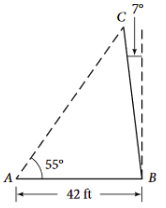
\includegraphics[scale=0.8]{figures/problem08.png}
\end{figure}

\end{document}
